%============================================================================%
%
%	DOCUMENT DEFINITION
%
%============================================================================%

%we use article class because we want to fully customize the page and dont use a cv template
\documentclass[10pt,A4]{article}	
%------------------------------------------------------------------------------------
%	ENCODING
%------------------------------------------------------------------------------------
%we use utf8 since we want to build from any machine
\usepackage[utf8]{inputenc}

%------------------------------------------------------------------------------------
%	LOGIC
%------------------------------------------------------------------------------------
% provides \isempty test
\usepackage{xifthen}

%------------------------------------------------------------------------------------
%	FONT
%------------------------------------------------------------------------------------

% some tex-live fonts - choose your own

%\usepackage[defaultsans]{droidsans}

%\usepackage[default]{raleway}
%\usepackage{fetamont}
%\usepackage[default]{gillius}
\usepackage[light,math]{iwona}
%\usepackage[thin]{roboto} 

% set font default
\renewcommand*\familydefault{\sfdefault} 	
\usepackage[T1]{fontenc}

% more font size definitions
\usepackage{moresize}		
\usepackage{fontawesome}
% \usepackage{fontawesome5}

%------------------------------------------------------------------------------------
%	PAGE LAYOUT  DEFINITIONS
%----------------------------------------------------------------------------------------

%debug page outer frames
%\usepackage{showframe}			


%define page styles using geometry
\usepackage[a4paper]{geometry}		

% for example, change the margins to 2 inches all round
\geometry{top=1cm, bottom=-.6cm, left=0.4cm, right=1cm} 	


%less space between header and content
\setlength{\headheight}{-5pt}		

%indentation is zero
\setlength{\parindent}{0mm}

%----------------------------------------------------------------------------------------
%	TABLE /ARRAY DEFINITIONS
%---------------------------------------------------------------------------------------- 

%for layouting tables
\usepackage{multicol}			
\usepackage{multirow}

%extended aligning of tabular cells
\usepackage{array}

%Tabular X 
\usepackage{tabularx}

\newcolumntype{x}[1]{%
>{\raggedleft\hspace{0pt}}p{#1}}%

%----------------------------------------------------------------------------------------
%	GRAPHICS DEFINITIONS
%---------------------------------------------------------------------------------------- 

%for header image
\usepackage{graphicx}

%for floating figures
\usepackage{wrapfig}
\usepackage{float}
%\floatstyle{boxed} 
%\restylefloat{figure}

%for drawing graphics		
\usepackage{tikz}				
\usetikzlibrary{shapes, backgrounds, mindmap, trees}

%----------------------------------------------------------------------------------------
%	Color DEFINITIONS
%---------------------------------------------------------------------------------------- 
\usepackage{transparent}
\usepackage{color}

%accent color
\definecolor{complcol}{RGB}{250,150,10}

%dark background color
\definecolor{bgcol}{RGB}{110,110,110}

%light background / accent color
\definecolor{softcol}{RGB}{225,225,225}

\definecolor{sectcol}{RGB}{0,120,150}

\definecolor{boldgrey}{RGB}{170,170,170}
\definecolor{boldblue}{RGB}{7,45,171}

\usepackage{hyperref}
\hypersetup{
    colorlinks=true,
    linkcolor=blue,
    filecolor=black,      
    urlcolor=sectcol,
}
%============================================================================%
%	DEFINITIONS
%============================================================================%

% returns minipage width minus two times \fboxsep
% to keep padding included in width calculations
\newcommand{\mpwidth}{\linewidth-\fboxsep-\fboxsep}
	

%----------------------------------------------------------------------------------------
% 	ARROW GRAPHICS in Tikz
%----------------------------------------------------------------------------------------


% a six pointed arrow poiting to the left
\newcommand{\tzlarrow}{(0,0) -- (0.2,0) -- (0.3,0.2) -- (0.2,0.4) -- (0,0.4) -- (0.1,0.2) -- cycle;}	 %chktex 8	

% include the left arrow into a tikz picture
% param1: fill color
%
\newcommand{\larrow}[1]
{\begin{tikzpicture}[scale=0.58]
	 \filldraw[fill=#1!100,draw=#1!100!black]  \tzlarrow
 \end{tikzpicture}
}

% a six pointed arrow poiting to the right
\newcommand{\tzrarrow}{ (0,0.2) -- (0.1,0) -- (0.3,0) -- (0.2,0.2) -- (0.3,0.4) -- (0.1,0.4) -- cycle;} %chktex 8	

% include the right arrow into a tikz picture
% param1: fill color
%
\newcommand{\rarrow}
{
\begin{tikzpicture}[scale=0.7]
	\filldraw[fill=sectcol!100,draw=sectcol!100!black] \tzrarrow
 \end{tikzpicture}
}

%----------------------------------------------------------------------------------------
%	custom sections
%----------------------------------------------------------------------------------------

% create a coloured box with arrow and title as cv section headline
% param 1: section title
%
\newcommand{\cvsection}[2]{
    \colorbox{sectcol}{\mystrut\makebox[1\mpwidth][l]{\hspace{1pt}\textcolor{white}{\csname fa#1\endcsname}\hspace{4pt} \textbf{\textcolor{white}{\uppercase{#2}}}\hspace{4pt}
}}\\
}

% create a coloured arrow with title as cv meta section section
% param 1: meta section title
%
\newenvironment{metasection}[1] {
	\vspace{6pt}
	\begin{center}
		\textcolor{black}{\large{\uppercase{#1}}}\\
	\normalsize
	\parbox{0.7\mpwidth}{\textcolor{black}	\hrule}
}{\end{center}}

%----------------------------------------------------------------------------------------
%	 CV EVENT
%----------------------------------------------------------------------------------------

% creates a stretched box as cv entry headline followed by two paragraphs about 
% the work you did
% param 1:	event time i.e. 2014 or 2011-2014 etc.
% param 2:	event name (what did you do?)
% param 3:	institution (where did you work / study)
% param 4:	what was your position
% param 5:	some words about your contributions
%
\newcommand{\eventbullet}{\hspace{-3.9pt}\small{\faDotCircleO} \hspace{5pt}}

\newcommand{\cvevent}[5]
{
\vspace{12pt}
	\begin{tabular*}{1\mpwidth}{p{0.45\mpwidth}  x{0.52\mpwidth}}
 	\textcolor{black}{\textbf{#2}} & \textcolor{complcol}{#3}, \textcolor{bgcol}{#1} 
	\end{tabular*}
\textcolor{softcol}{\hrule}
\vspace{6pt}
	\begin{tabular*}{0.5\mpwidth}{p{\mpwidth}}
        \larrow{softcol}  #4\\[3pt]
        \larrow{softcol}  #5\\[6pt]
	\end{tabular*}
}

% 1 - Title
% 2 - Year
% 3 - Institution
% 4 - Place
% 5 - Description 1
% 6 - Description 2

\newcommand{\newcvevent}[6]
{
	\begin{tabular*}{1\mpwidth}{p{0.68\mpwidth}  x{0.27\mpwidth}}
		\textcolor{sectcol}{#1} & \textcolor{sectcol}{#2}
	\end{tabular*}
	\begin{tabular*}{1\mpwidth}{p{0.65\mpwidth}  x{0.30\mpwidth}}
		{\textit{#3}} & {#4}
	\end{tabular*}
	\begin{tabular*}{0.5\mpwidth}{p{\mpwidth}}
		\larrow{softcol}  #5\\[3pt]
		\larrow{softcol}  #6\\[6pt]
    \end{tabular*} 
	\vspace{8pt}
}

\newcommand{\customicon}[2]{
	\hspace{87pt}{\csname fa#1\endcsname}\hspace{2pt}{#2}
}

% creates a stretched box as 
\newcommand{\cveventmeta}[2]
{
	\mbox{\mystrut\hspace{87pt}\textit{#1}}\\
	#2
}

%----------------------------------------------------------------------------------------
% CUSTOM STRUT FOR EMPTY BOXES
%----------------------------------------- -----------------------------------------------
\newcommand{\mystrut}{\rule[-.3\baselineskip]{0pt}{\baselineskip}}

%----------------------------------------------------------------------------------------
% CUSTOM LOREM IPSUM
%----------------------------------------------------------------------------------------
\newcommand{\lorem}
{Lorem ipsum dolor sit amet, consectetur adipiscing elit. Donec a diam lectus.}


% use to vertically center content
% credits to: http://tex.stackexchange.com/questions/7219/how-to-vertically-center-two-images-next-to-each-other
\newcommand{\vcenteredinclude}[1]{\begingroup
\setbox0=\hbox{\includegraphics{#1}}%
\parbox{\wd0}{\box0}\endgroup}

% use to vertically center content
% credits to: http://tex.stackexchange.com/questions/7219/how-to-vertically-center-two-images-next-to-each-other
\newcommand*{\vcenteredhbox}[1]{\begingroup
\setbox0=\hbox{#1}\parbox{\wd0}{\box0}\endgroup}

%----------------------------------------------------------------------------------------
%	ICON-SET EMBEDDING
%---------------------------------------------------------------------------------------- 

\newcommand{\icon}[3]{\makebox(#2, #2){\textcolor{#3}{\csname fa#1\endcsname}}}	%icon shortcut
\newcommand{\icontext}[4]{ 						%icon with text shortcut
	\vcenteredhbox{\icon{#1}{#2}{#4}} \vcenteredhbox{\textcolor{#4}{#3}}
}

\newcommand{\name}{Ricardo Jorge de Ara\'ujo Ferreira}
\newcommand{\email}{\email{ricarraf@gmail.com}}
\newcommand{\github}{\href{url}{https://github.com/ricarraf}}
\newcommand{\linkedin}{\href{www.linkedin.com/in/RicardoAraujoFerreira}{/RicardoAraujoFerreira}}



\newcommand{\identcontent}{\hspace{6pt}}

%============================================================================%
%
%	DOCUMENT CONTENT
%
%============================================================================%
\begin{document}
\fcolorbox{white}{white}{\begin{minipage}[c][0.95\textheight][t]{0.30\linewidth}

%
\begin{center}
	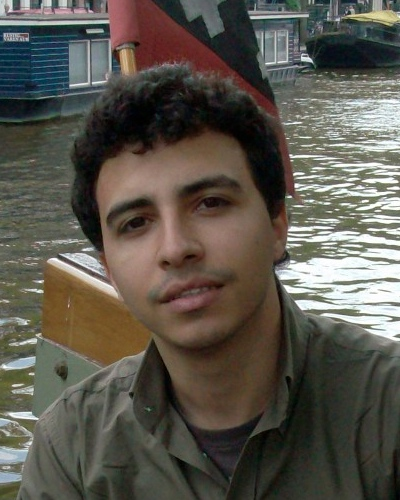
\includegraphics[width=0.45\mpwidth]{img/picture}
\end{center}

\begin{metasection}{Contact}

	\icontext{MapMarker}{12}{Porto, Portugal}{black}\\[6pt]
	\icontext{MobilePhone}{12}{+351 91 615 15 65}{black}\\[6pt]
	\icontext{Send}{12}{ricarraf@gmail.com}{black}\\[6pt]
	\icontext{Github}{12}{github.com/ricardojaferreira}{black}\\[6pt]
	\icontext{Linkedin}{12}{\linkedin}{black}\\[6pt]

\end{metasection}
%---------------------------------------------------------------------------------
%	META SECTION
%--------------------------------------------------------------------------------

\begin{metasection}{Programming Languages}
	\begin{tabular}{ll}
		JAVA & \icon{Star}{12}{complcol}\icon{Star}{12}{complcol}\icon{Star}{12}{complcol}\icon{Star}{12}{complcol}\icon{Star}{12}{black}\\[6pt]
		PHP & \icon{Star}{12}{complcol}\icon{Star}{12}{complcol}\icon{Star}{12}{complcol}\icon{Star}{12}{complcol}\icon{Star}{12}{black}\\[6pt]
		JavaScript & \icon{Star}{12}{complcol}\icon{Star}{12}{complcol}\icon{Star}{12}{complcol}\icon{Star}{12}{complcol}\icon{Star}{12}{black}\\[6pt]
		C\textbackslash C++ & \icon{Star}{12}{complcol}\icon{Star}{12}{complcol}\icon{Star}{12}{complcol}\icon{Star}{12}{black}\icon{Star}{12}{black}\\[6pt] %chktex 1	
		Python & \icon{Star}{12}{complcol}\icon{Star}{12}{complcol}\icon{Star}{12}{black}\icon{Star}{12}{black}\icon{Star}{12}{black}\\[6pt] %chktex 1	
	\end{tabular}
\end{metasection}


\begin{metasection}{Technologies}

	\textcolor{black}{
        PlayFramework {\tiny \icon{Circle}{6}{black}} Spring {\scriptsize \faCircle} Zend Famework {\tiny \icon{Circle}{6}{black}} Angular {\scriptsize \faCircle} Apache {\scriptsize \faCircle} Nginx {\scriptsize \faCircle} Git {\scriptsize \faCircle} MySql / MariaDB {\scriptsize \faCircle} MongoDB {\scriptsize \faCircle} ElasticSearch {\scriptsize \faCircle} Couchbase {\scriptsize \faCircle} RabbitMQ {\scriptsize \faCircle} \LaTeX %chktex 1	
	}
\end{metasection}

		\begin{metasection}{Languages}
	\begin{tabular}{ll}
		Portuguese & \icon{Star}{12}{complcol}\icon{Star}{12}{complcol}\icon{Star}{12}{complcol}\icon{Star}{12}{complcol}\icon{Star}{12}{complcol}\\[6pt]
		Italian & \icon{Star}{12}{complcol}\icon{Star}{12}{complcol}\icon{Star}{12}{complcol}\icon{Star}{12}{complcol}\icon{Star}{12}{complcol}\\[6pt]
		English & \icon{Star}{12}{complcol}\icon{Star}{12}{complcol}\icon{Star}{12}{complcol}\icon{Star}{12}{complcol}\icon{Star}{12}{black}\\[6pt]
	\end{tabular}
\end{metasection}

\begin{metasection}{Operating Systems}

	\textcolor{white}{\LARGE{\icon{Apple}{24}{black} \icon{Linux}{24}{black} \icon{Windows}{24}{black}}}

\end{metasection}

\begin{metasection}{Activities}
	\\
	\textcolor{black}{\large{\icon{Plane}{20}{black} \icon{Headphones}{20}{black}  \icon{Bicycle}{20}{black} \icon{Laptop}{20}{black}}}
\end{metasection}

\begin{center}
    See the extended version at \href{https://git.io/fhQUd}{https://git.io/fhQUd}.
\end{center}

\end{minipage}}%
\fcolorbox{white}{white}{\begin{minipage}[c][0.95\textheight][t]{0.72\linewidth}


%-----------------------------------------------------------------------------------
%	TITLE HEADLINE
%-----------------------------------------------------------------------------------
\vspace{-3pt}
%-----------------------------------------------------------------------------------
%	HEADER IMAGE
%----------------------------------------------------------------------------------


%\hspace{-1.6cm}
%\includegraphics[trim= 0 250 0 270,clip,width=1\linewidth+3.1cm]{myfoto.jpg}	%trimming relative to image size!
%\includegraphics[trim= 350 150 0 200, clip ,width=\linewidth]{myfoto.jpg}	%trimming relative to image size

%---------------------------------------------------------------------------------------
%	SUMMARY
%----------------------------------------------------------------------------------------
\textbf{\huge \name} \\
\Large Electrical and Computer Science Engineer (M.Sc.) \\
\large Student of Master in Informatics and Computing Engineering \\
%
%============================================================================%
%
%	CV SECTIONS AND EVENTS (MAIN CONTENT)
%
%============================================================================%

%----------------------------------------------------------------------------------
%	STATUS
%----------------------------------------------------------------------------------
\cvsection{User}{Summary}

\begin{tabular*}{1.0\mpwidth}{@{\identcontent}| p{0.97\mpwidth}} %chktex 44	
	\vspace{0.1pt}
	I am currently working has a full stack developer in an Agile (scrum) environment with modern technologies, previleging good quality code and architectures. To learn more about software development, I have started the Master Degree in Informatics and Computing Engineering at Faculdade de Engenharia, I am currently at the 4rd year out of a 5 year program.
\end{tabular*}

\vspace{12pt}

%----------------------------------------------------------------------------------
%	EXPERIENCE
%----------------------------------------------------------------------------------
\cvsection{Briefcase}{Experience}

\begin{tabular*}{0.5\mpwidth}{@{\identcontent}|@{\eventbullet} p{0.97\mpwidth}} %chktex 44
	\newcvevent{Web Engineer - Fullstack Developer}{2018/06 - now}{Jumia - Porto Tech Center}{Porto, Portugal}{Development of web applications using JAVA and PHP frameworks;}{Analysis and implementation of new software solutions.} %chktex 8
	\\
    \newcvevent{Web Engineer - Fullstack Developer}{2018/02 - 2018/06}{7Skin, Lda - Ecommerce}{Porto, Portugal}{Development of ecommerce solutions using Magento;}{Development of internal software to improve productivity.} %chktex 8
	\\
    \newcvevent{Web Engineer - Fullstack Developer}{2014/05 - 2018/02}{GravityDemand, Lda - Ecommerce}{Penafiel, Portugal}{Development of software for ecommerce and marketing solutions;}{Development and integration with external services (REST and other API's).} %chktex 8
	\\
    \newcvevent{R\&D - Engineer}{2011/01 - 2011/09}{INESC - Institute for System and Computer Engineering}{Porto, Portugal}{Research and testing in the power energy field (software and hardware);}{Validate emerging concepts in Smart-Grids with prototypes and models.} %chktex 8
	\\
    \newcvevent{Automation Engineer}{2008/08 - 2011/01}{Efacec, Sistemas de Engenharia}{Maia, Portugal}{Development of control and automation systems;}{Management of large information systems based on UNIX platforms.} %chktex 8
\end{tabular*} 


\vspace{12pt}
% %---------------------------------------------------------------------------------------
% %	EDUCATION SECTION
% %--------------------------------------------------------------------------------------
\cvsection{GraduationCap}{Education}

\begin{tabular*}{0.5\mpwidth}{@{\identcontent}|@{\eventbullet} p{0.97\mpwidth}} %chktex 44
	\newcvevent{M.Sc.\ in Informatics and Computation Engineering}{Present}{Faculdade de Eng.\ da Universidade do Porto}{Porto, Portugal}{Currently at the 4rd Year, 2 more to finish the graduation.}{.}
	\\
	\newcvevent{M.Sc.\ in Electrical and Computers Engineering}{Present}{Faculdade de Eng.\ da Universidade do Porto}{Porto, Portugal}{Specialization: Automation and Control Systems}{Thesis: Solar Car - Control and development. (17 out of 20)} %chktex 8
\end{tabular*}


\end{minipage}}

%-------------------------------------------------------------------------------------------------
%	ARTIFICIAL FOOTER (fancy footer cannot exceed linewidth) 
%--------------------------------------------------------------------------------------------------

\null %chktex 1
\vspace*{\fill}
\hspace{-0.25\linewidth}\colorbox{bgcol}{\makebox[1.5\linewidth][c]{\mystrut\small \textcolor{white}{Resume 2019 | Ricardo Ferreira :: ricarraf@gmail.com} $\cdot$ \textcolor{white}{:: 916 151 56 5}}}

%============================================================================%
%	DOCUMENT END
%============================================================================%
\end{document}

